\documentclass{article}
\usepackage{graphicx} % Required for inserting images
\usepackage{amsmath}
\usepackage{caption}
\usepackage{booktabs}
\usepackage[table,xcdraw]{xcolor}
\usepackage{changepage}

\usepackage[backend=biber, style=apa, citestyle=apa]{biblatex}
\addbibresource{references.bib}

\usepackage[a4paper, total={6.5in, 9.5in}]{geometry}
\title{Financial Modelling Individual Project}
\author{Elliott Oates}
\date{December 2023}
\setlength{\parskip}{\baselineskip}


\begin{document}



\maketitle

Word count: 1575 max 

\newpage\section*{What is the objective of the case study and what are the main conclusions?}
The objective was to compare the profitability of momentum trading strategies built on moving averages for an equally weighted portfolio of G10 currencies. The outset of the case study required calculating monthly returns as in (\ref{eq:1}) for data containing monthly exchange rates between Jan 1993 - Oct 2021 for the USD against the remaining G10 currencies (GBP, CAD, JPY, AUD, NZD, SEK, NOK, CHF and EUR). The exchange rates are quoted as the number of USD per 1 Foreign Currency Unit (FCU).  $C_{t+1}$ is the return from investing in a foreign currency between month $t$ and month $t+1$ where $S_{t}$ and $S_{t+1}$ are the FCU/USD exchange rate at time $t$ and $t+1$ respectively. The data are monthly returns but we do not know if the data represents month-end, month start or monthly averages. 

\begin{equation}\label{eq:1}
    C_{t+1}=\frac{S_{t+1}-S_{t}}{S_{t}} = \frac{S_{t+1}}{S_{t}}-1
\end{equation}

We then compute the long run, $\overline{C}_{t,L}$, and short run ,$\overline{C}_{t,S}$, moving averages for each exchange rate at month $t$ with (\ref{eq:2}) and (\ref{eq:3}) respectively, where $n$ represents the long run window and $m$ represents the short run window. 

\begin{minipage}{0.45\textwidth}
\begin{equation}\label{eq:2}
    \overline{C}_{t,L} = \frac{1}{n}\sum_{i=0}^{n-1} S_{t-1}
\end{equation}
\end{minipage}
\hfill
\begin{minipage}{0.45\textwidth}
\begin{equation}\label{eq:3}
    \overline{C}_{t,S}= \frac{1}{m}\sum_{i=0}^{m-1} S_{t-1}
\end{equation}
\end{minipage}

\begin{figure}[h!]
    \centering
    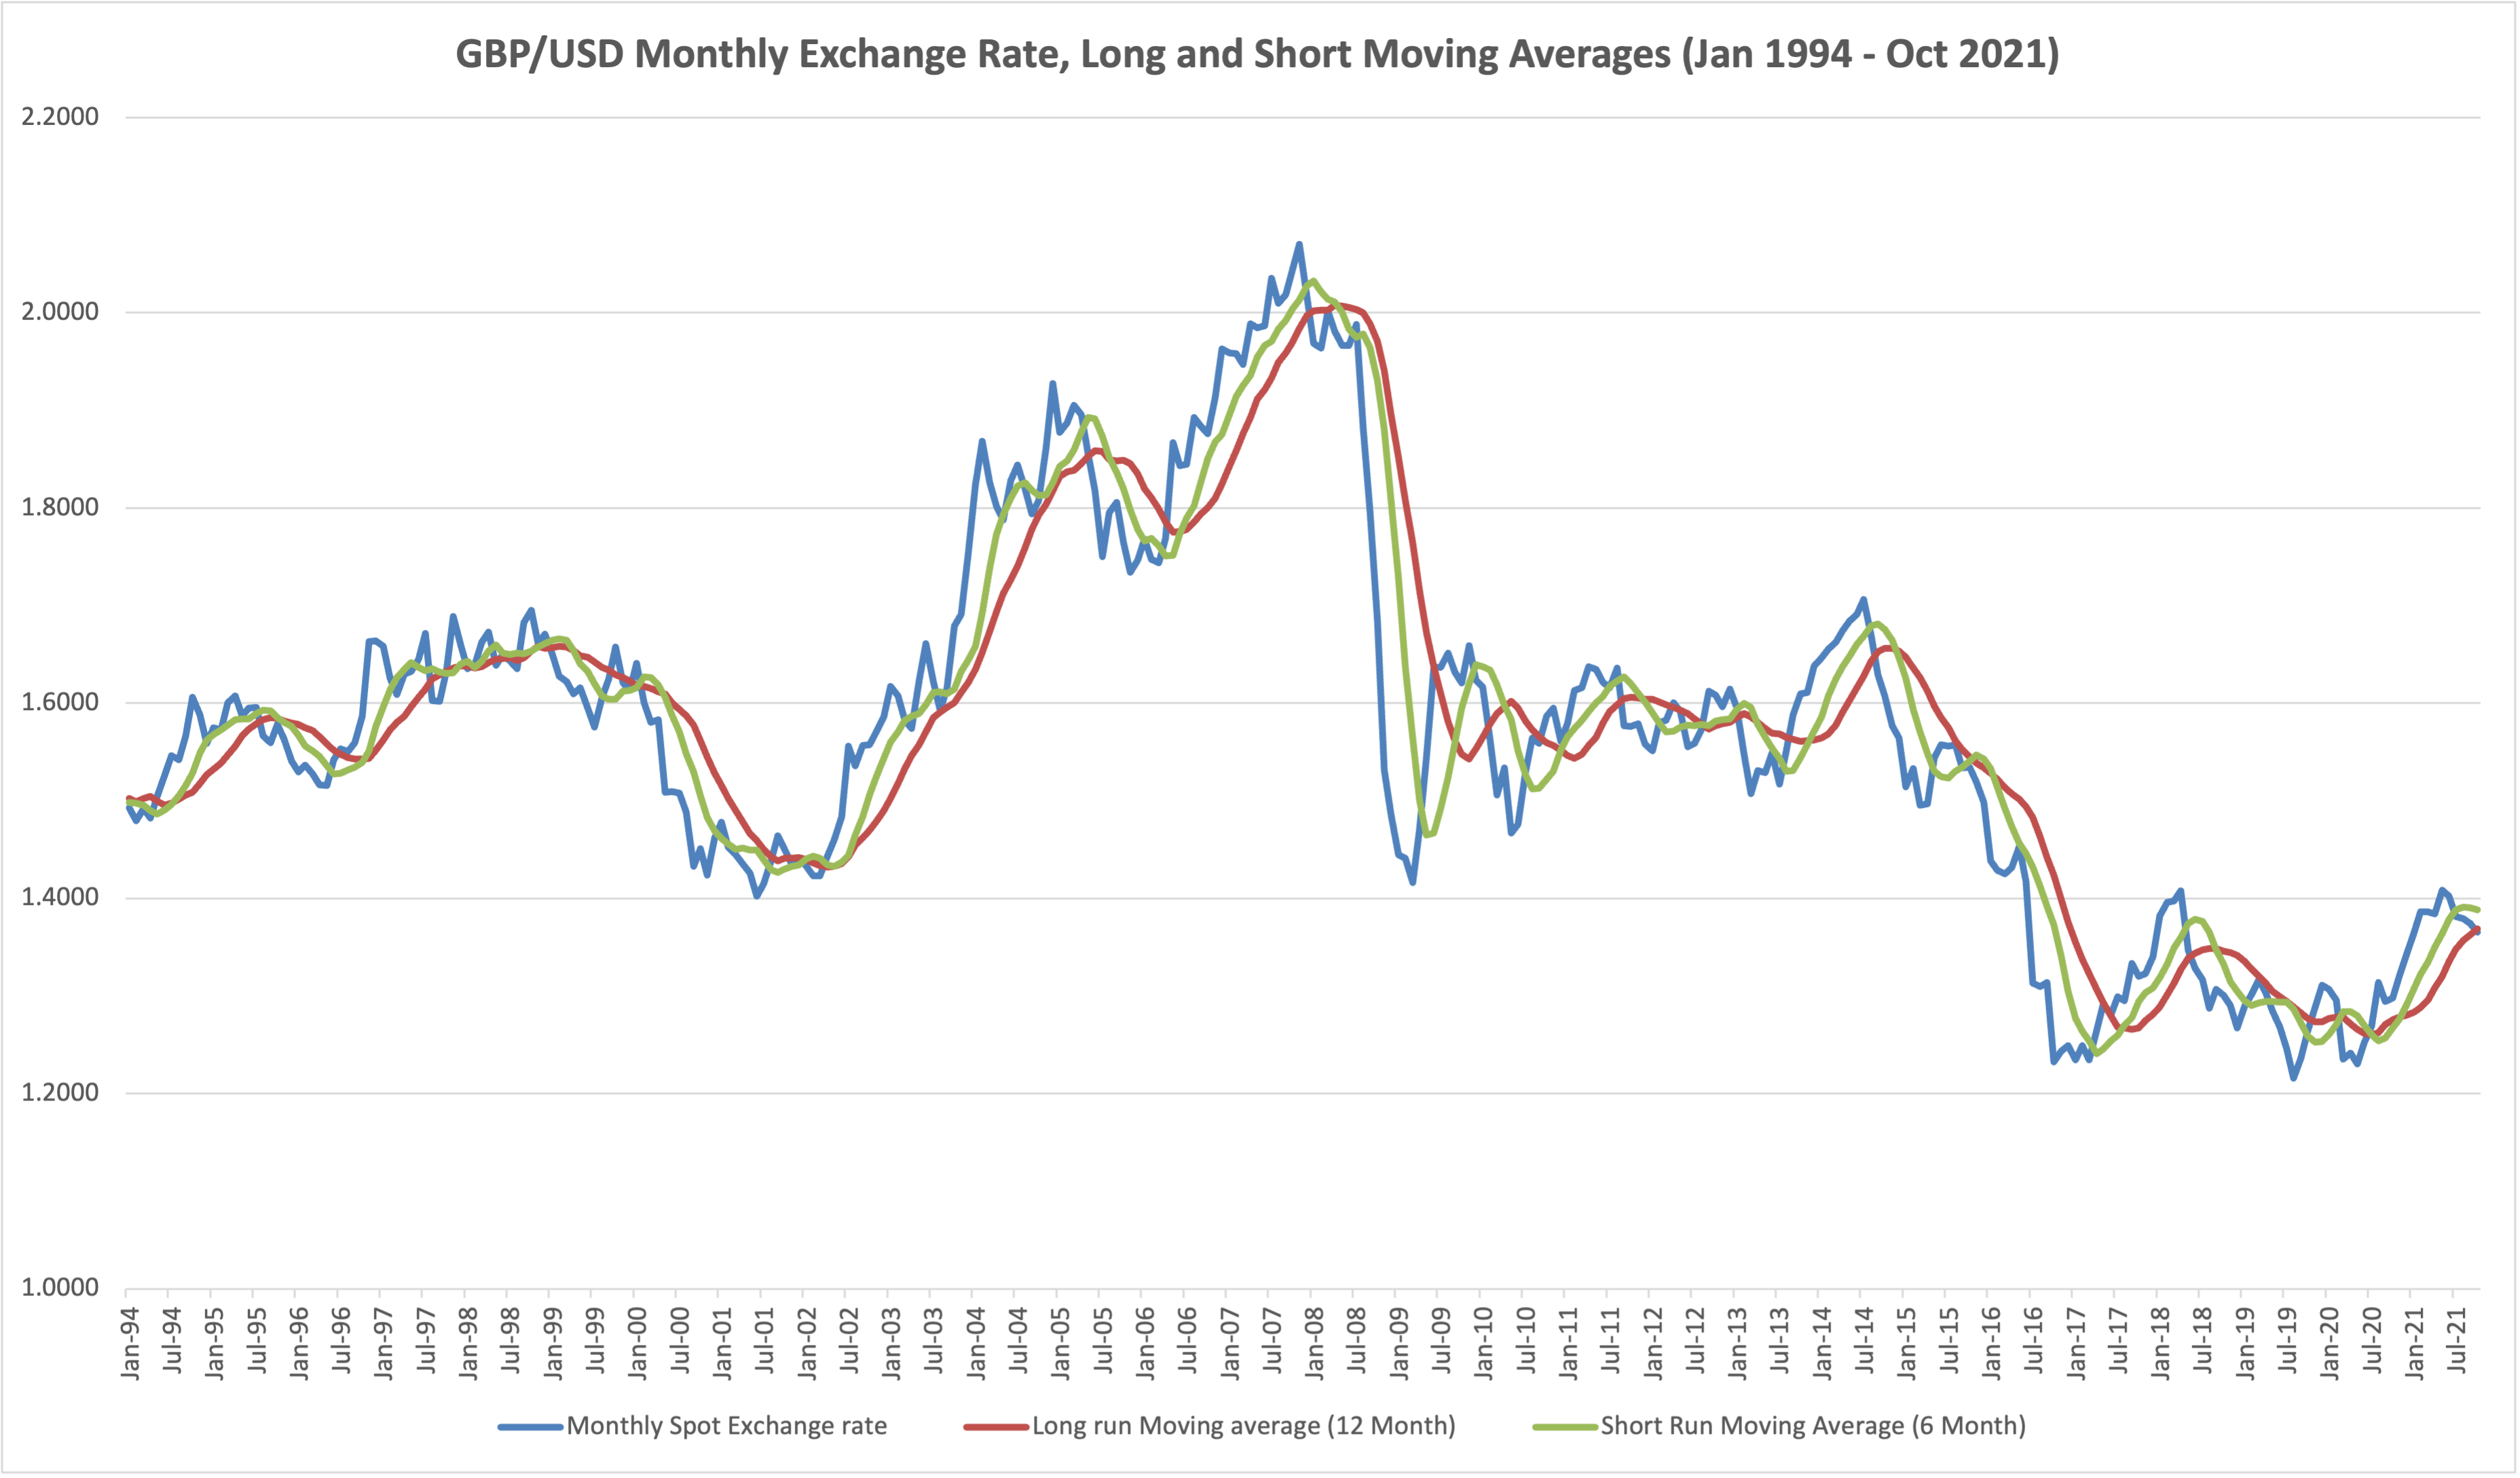
\includegraphics[width=0.75\linewidth]{GBP_USD Rates.png}
    \captionsetup{font=small, width = 0.75\linewidth}
    \caption{\centering GBP/USD Monthly Spot Exchange rate, Long Run Moving Average $\overline{C}_{t,L}$ with $m = 12$  and Short Run Moving Average $\overline{C}_{t,S} $ with $ n = 6$}
    \label{fig:GBP/USD}
\end{figure}

With both moving averages computed such as the one for the GBP/USD exchange shown in figure \ref{fig:GBP/USD} for each FCU/USD pairing, we design our momentum trading strategy. The US investor compares the a short run and long run moving averages of each exchange rate and accordingly will go long if the short run moving average is higher than the long run and will go short vice versa. This strategy assumes one can exploit short run trends in the exchange rate and that if the rate has increased recently it is likely to increase further in the near future. These trends, if they exist, arise from investors’ behavioural biases and represent a deviation from market efficiency. The strategy can be represented algebraically as in (\ref{eq:4}).

\begin{equation}\label{eq:4}
MA(m,n) = \frac{1}{m}\sum_{i=0}^{m-1} S_{t-1} - \frac{1}{n}\sum_{i=0}^{n-1} S_{t-1}
\end{equation}
\[
\text{where  } m < n
\]

The momentum return at month $t$ for a currency position is the simple return if the US investor will buy the currency that month given $MA(m,n)>0$ or if $MA(m,n) < 0$ the investor will sell the currency and earn the negative of the simple return. The case study prescribed investigating the trading strategy on a equally weighted portfolio of all G10 currencies we calculate portfolio monthly returns as the average of all the individual positions. Initialising a portfolio with arbitrary value of 100 in December 1993, we can observe how the portfolio value changes over time. Figure \ref{fig:Portfolio Values} compares the momentum portfolio with a passively managed equal-weighted portfolio where returns are the average simple return of each position. We can calculate the metrics in Table \ref{table:1} to compare profitability and risk of both portfolios. 

\begin{figure}[h!]
    \centering
    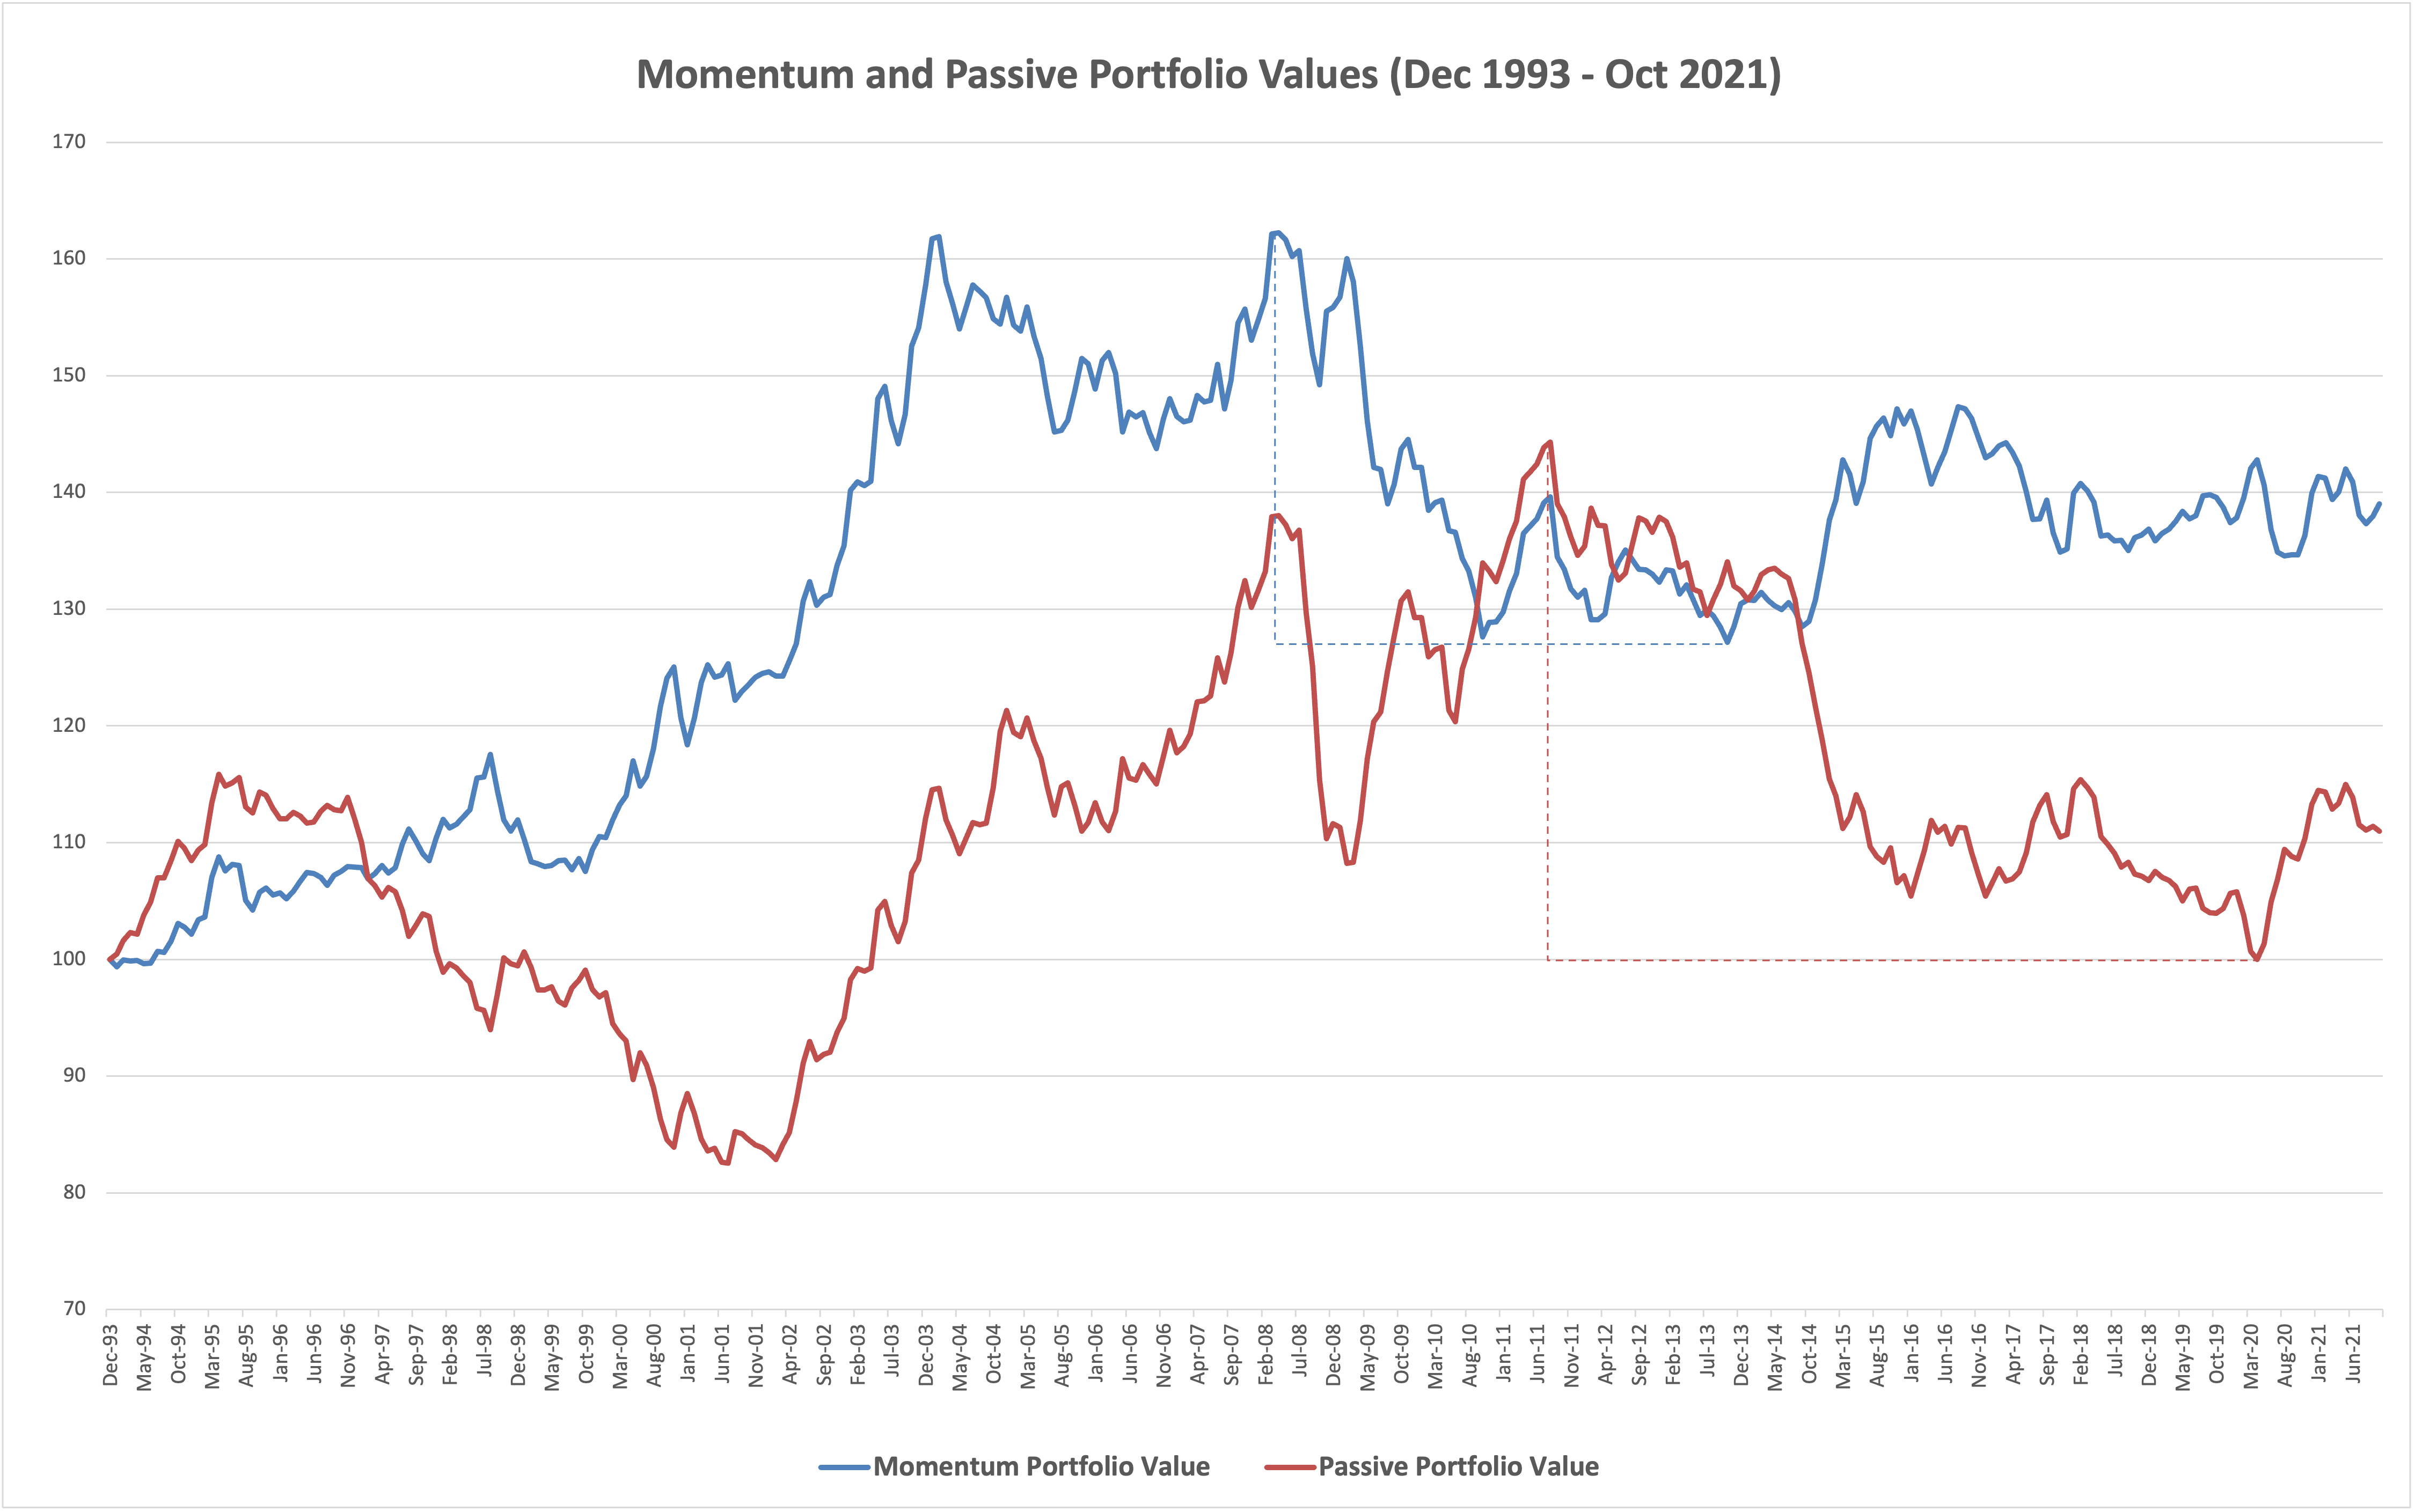
\includegraphics[width=0.75\linewidth]{Figure 2.png}
    \captionsetup{font=small, width = 0.75\linewidth}
    \caption{Momentum (6,12) traded and passively managed portfolio values over time. Maximum Drawdown for each portfolio is indicated with dashed line. }
    \label{fig:Portfolio Values}
\end{figure}

\begin{table}[h!]
    \centering
    \captionsetup{font=small,width =0.5\linewidth}
    \caption{\centering Performance Metrics for Momentum and Passive Strategies}
    \label{table:1}
    \begin{tabular}{lccc}
        \toprule
        & \textbf{Momentum} & \textbf{Passive} \\
        \midrule
        Average return & 0.11\% & 0.05\% \\
        SD & 1.41\% & 1.75\% \\
        Sharpe ratio & 0.077 & 0.027 \\
        Maximum drawdown & 21.62\% & 30.71\% \\
        \bottomrule
    \end{tabular}
\end{table}

The expected monthly return for the momentum ($6,12$) portfolio is $0.11\%$ (2d.p.). It is evident that simple active strategies exceed expected returns from a passively managed portfolio. The standard deviation, which describes the average deviation of returns from the mean return is lower for the momentum portfolio indicating less volatility. As a first measure of risk adjusted returns we compute the Sharpe ratio for with equation (\ref{eq:5}). While more will be said about the validity of the sharpe ratios, the higher value for the momentum portfolio suggests a higher risk adjusted performance for the momentum ($6,12$) than the passive portfolio. The maximum drawdown, the largest cumulative reduction in portfolio value, $V_{t}$, over a period of time is calculated via equation (\ref{eq:6}) and also favours the momentum portfolio. 

\begin{equation}\label{eq:5}
    S_{p}=\frac{E(R_{p})-R_{f}}{\sigma_{p}}=\frac{E(R_{p})}{\sigma_{p}}
\end{equation}

\begin{equation}\label{eq:6}
        MDD = \text{max}_{t=1,...,T}\frac{-(V_{t}-\text{max}_{i=1,...,t-1}(V_{t-i}))}{(\text{max}_{i}(V_{t-i})}
\end{equation}

Its established that our momentum ($6,12$) filter can provide better risk adjusted returns than a passively managed portfolio. However our goal is to investigate a class of momentum strategies to find the optimal window length parameters by conducting a sensitivity analysis to find the Sharpe ratios for portfolios managed with different parameters. From table 2 we observe that the largest sharp ratio and thus the best risk adjusted monthly returns would be achieved with our momentum strategy with a 1 month short, 2 month long window.
\begin{table}[h!]
\centering
\captionsetup{font=small, width = 0.9\linewidth}
\caption{\centering Sharpe Ratios for Momentum Strategies Monthly Returns with Varying Window Lengths for an Equally Weighted G10/USD Portfolio (Dec 1993 - Oct 2021)}
\label{tab:2}
\resizebox{0.9\textwidth}{!}{%
\begin{tabular}{rlllllllllll}
\multicolumn{1}{l}{} &
  \textbf{} &
  \textbf{} &
   &
  \multicolumn{4}{l}{\textbf{$n$ (Long Window)}} &
   &
   &
   &
   \\ \cline{2-12} 
\multicolumn{1}{c|}{\textbf{\begin{tabular}[c]{@{}c@{}}$m$ (Short \\ Window)\end{tabular}}} &
  \multicolumn{1}{c}{2} &
  \multicolumn{1}{c}{3} &
  \multicolumn{1}{c}{4} &
  \multicolumn{1}{c}{5} &
  \multicolumn{1}{c}{6} &
  \multicolumn{1}{c}{7} &
  \multicolumn{1}{c}{8} &
  \multicolumn{1}{c}{9} &
  \multicolumn{1}{c}{10} &
  \multicolumn{1}{c}{11} &
  \multicolumn{1}{c}{12} \\ \cline{2-12} 
\multicolumn{1}{r|}{1} &
  \cellcolor[HTML]{63BE7B}0.412 &
  \cellcolor[HTML]{9FD07F}0.297 &
  \cellcolor[HTML]{A2D07F}0.292 &
  \cellcolor[HTML]{ADD480}0.272 &
  \cellcolor[HTML]{B3D680}0.258 &
  \cellcolor[HTML]{BCD881}0.242 &
  \cellcolor[HTML]{BDD881}0.240 &
  \cellcolor[HTML]{C7DB81}0.222 &
  \cellcolor[HTML]{CFDE82}0.205 &
  \cellcolor[HTML]{CCDD82}0.211 &
  \cellcolor[HTML]{D1DE82}0.203 \\
\multicolumn{1}{r|}{2} &
   &
  \cellcolor[HTML]{D2DE82}0.199 &
  \cellcolor[HTML]{E5E483}0.164 &
  \cellcolor[HTML]{E3E383}0.168 &
  \cellcolor[HTML]{E5E483}0.163 &
  \cellcolor[HTML]{E8E583}0.159 &
  \cellcolor[HTML]{EFE784}0.144 &
  \cellcolor[HTML]{F4E884}0.134 &
  \cellcolor[HTML]{F8E984}0.126 &
  \cellcolor[HTML]{F5E884}0.134 &
  \cellcolor[HTML]{F3E884}0.136 \\
\multicolumn{1}{r|}{3} &
   &
   &
  \cellcolor[HTML]{FCEB84}0.119 &
  \cellcolor[HTML]{FEE783}0.110 &
  \cellcolor[HTML]{F3E884}0.136 &
  \cellcolor[HTML]{F2E884}0.138 &
  \cellcolor[HTML]{FBEA84}0.121 &
  \cellcolor[HTML]{FEE482}0.108 &
  \cellcolor[HTML]{FEDA80}0.101 &
  \cellcolor[HTML]{FEDF81}0.104 &
  \cellcolor[HTML]{FCEA84}0.119 \\
\multicolumn{1}{r|}{4} &
   &
   &
   &
  \cellcolor[HTML]{F7E984}0.129 &
  \cellcolor[HTML]{EDE683}0.148 &
  \cellcolor[HTML]{F6E984}0.131 &
  \cellcolor[HTML]{FEEB84}0.115 &
  \cellcolor[HTML]{FDC77D}0.086 &
  \cellcolor[HTML]{FCC17B}0.082 &
  \cellcolor[HTML]{FDCC7E}0.090 &
  \cellcolor[HTML]{FEDC81}0.102 \\
\multicolumn{1}{r|}{5} &
   &
   &
   &
   &
  \cellcolor[HTML]{F0E784}0.142 &
  \cellcolor[HTML]{F7E984}0.129 &
  \cellcolor[HTML]{FEEB84}0.116 &
  \cellcolor[HTML]{FDCF7E}0.092 &
  \cellcolor[HTML]{FBA276}0.059 &
  \cellcolor[HTML]{FBAD78}0.067 &
  \cellcolor[HTML]{FCBD7B}0.079 \\
\multicolumn{1}{r|}{6} &
   &
   &
   &
   &
   &
  \cellcolor[HTML]{FDCA7D}0.089 &
  \cellcolor[HTML]{FCC57C}0.085 &
  \cellcolor[HTML]{FBB078}0.069 &
  \cellcolor[HTML]{F98B71}0.042 &
  \cellcolor[HTML]{FA9E75}0.055 &
  \cellcolor[HTML]{FCBB7A}0.077 \\
\multicolumn{1}{r|}{7} &
   &
   &
   &
   &
   &
   &
  \cellcolor[HTML]{FCBF7B}0.080 &
  \cellcolor[HTML]{FBA376}0.059 &
  \cellcolor[HTML]{F98E72}0.043 &
  \cellcolor[HTML]{F98871}0.039 &
  \cellcolor[HTML]{FCBE7B}0.079 \\
\multicolumn{1}{r|}{8} &
   &
   &
   &
   &
   &
   &
   &
  \cellcolor[HTML]{FA9473}0.048 &
  \cellcolor[HTML]{F97C6E}0.030 &
  \cellcolor[HTML]{F98570}0.037 &
  \cellcolor[HTML]{FBAE78}0.067 \\
\multicolumn{1}{r|}{9} &
   &
   &
   &
   &
   &
   &
   &
   &
  \cellcolor[HTML]{F8696B}0.016 &
  \cellcolor[HTML]{F97C6E}0.030 &
  \cellcolor[HTML]{FA9974}0.052 \\
\multicolumn{1}{r|}{10} &
   &
   &
   &
   &
   &
   &
   &
   &
   &
  \cellcolor[HTML]{FA9072}0.045 &
  \cellcolor[HTML]{FBA977}0.063 \\
\multicolumn{1}{r|}{11} &
   &
   &
   &
   &
   &
   &
   &
   &
   &
   &
  \cellcolor[HTML]{FA8F72}0.045
\end{tabular}%
}
\end{table}

When $m = 1, n=2$ the momentum strategy amounts to buying if this period’s exchange rate is higher than last period’s exchange rate, and selling if this period’s exchange rate is lower than last period’s exchange rate. Table \ref{tab:3} and Figure 4 prove that a portfolio managed under these parameters is superior to others considered so far. Additionally conducting a sensitivity analysis for both the expected monthly returns and maximum portfolio drawdowns confirm that this strategy is optimal when back tested on our historical data (see Appendix A and Appendix B).


\begin{table}[h]
    \small % Set the font size to small
    \begin{minipage}{0.3\linewidth}
        \begin{adjustwidth}{-0.1cm}{}
            \centering
            \captionsetup{font = footnotesize}
            \caption{\centering Performance Metrics for Momentum Strategy ($n=11,m=2$)}
            \label{table:performance2}
            \begin{tabular}{lc}
                \toprule
                & \textbf{Momentum} \\
                \midrule
                Average return & 0.53\% \\
                SD & 1.29\% \\
                Sharpe ratio & 0.412 \\
                Maximum drawdown & 3.95\% \\
                \bottomrule
            \end{tabular}
        \end{adjustwidth}
    \end{minipage}%
    \hspace{\fill} % Add horizontal space between minipages
    \begin{minipage}{0.6\linewidth} % Adjust the width of the second minipage
        \begin{adjustwidth}{+1cm}{}
            \centering
            \label{fig:3}
            \captionsetup{font=footnotesize,width=\linewidth}
            \caption*{\centering Figure 3: Comparison of momentum(1,2) portfolio value over time with momentum (6,12) and passive portfolio}
            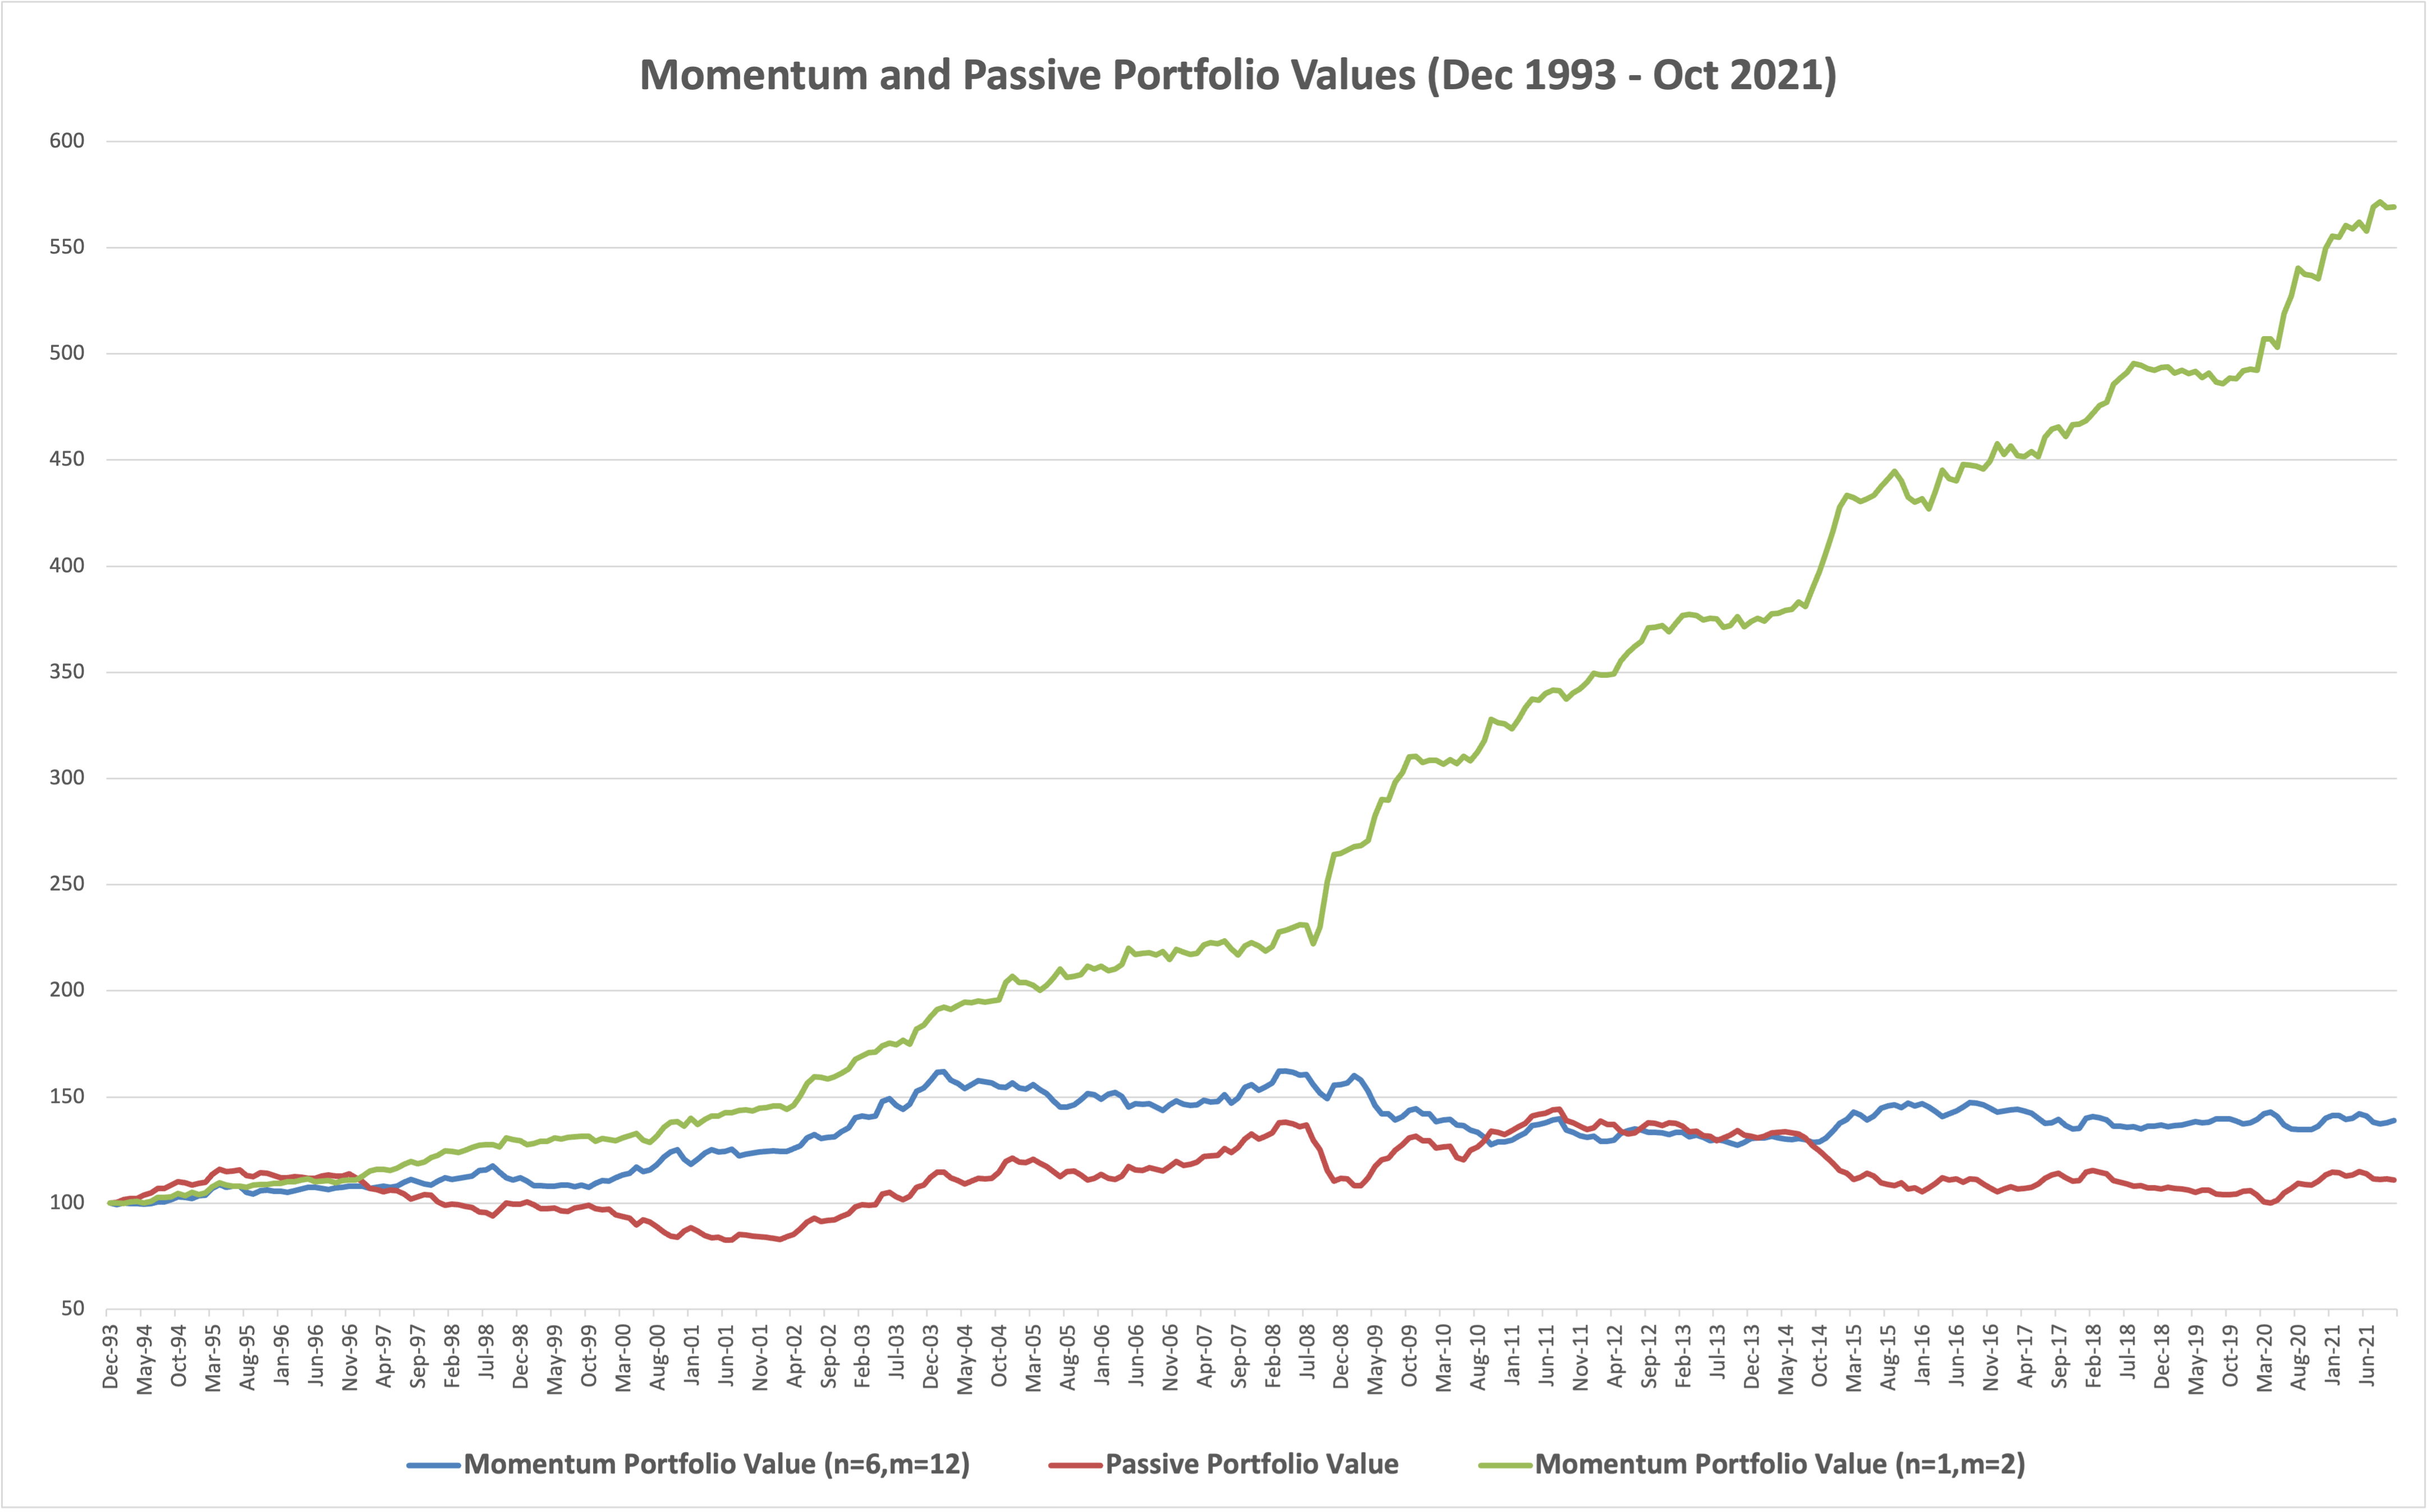
\includegraphics[width=\linewidth]{Figure 3.png}
        
        \end{adjustwidth}
    \end{minipage}
\end{table}

\newpage\section*{How would a practitioner make use of the findings of the case study?}

Deutsche-Bank, winners of this year Euromoney FX's award for best global FX provider, considers momentum trading as one of the top 3 most extensively used FX investment strategies (\cite{EUROMONEY_2023,deutschebank_2009}). Tasked with the role of a quantitative analyst responsible for designing strategies for FX traders to implement we devise a momentum strategy that is elementary compared to industry standards. Yet since individual strategies are subject to alpha decay and profitability is rarely everlasting the case study is beneficial in learning to develop sufficiently general methodologies and frameworks that enable quantitative analysts to generate new trading strategies and adapt existing ones quickly. After designing a class family of momentum trading strategies, buy if $MA(m,n)>0$ or sell if $MA(m,n) < 0$ we back-test the strategies on historical data which is similar to how p-measure quants spend a vast amount of their time (\cite{efinancialCareers2023}).

Several different roles in an investment bank would use the findings. Quantitative researchers would perhaps shift their focus into developing and using strategies that generate $\alpha$ (excess returns) smaller moving average windows given the superiority of the ($1,2$) strategy. FX markets are the world's largest and most liquid (\cite{investopedia}). Since they are also open 24 hours a day, from Sunday evening to Friday night, momentum strategies could probably be more profitable at the weekly, daily and even inter-day windows. An FX product salesperson could present the immense portfolio value growth to prospective clients, persuading them to invest with the bank. Portfolio managers in client funds could use the case study findings to communicate the expected performance and risks associated with different momentum strategies to clients. A risk manager uses historical volatility to evaluate value at risk. 

\section*{What are the limitations of the modelling approaches used in the case study?}
\subsubsection*{Interest Rates}
The omission of interest rates significantly limits our approach. In practice, domestic and foreign interest rates both come into play. For a US investor the currency return remains as in (\ref{eq:1}) but the investor will earn interest on the foreign deposit at rate $r_{t}^{*}$ and so the total monthly return is given by (\ref{eq:7}). Since our approach ignored the return from the foreign deposit it potentially underestimates the portfolios monthly returns. Furthermore if the investor borrows at rate $r_{t}$ to finance the portfolios position, the portfolios excess return is given by (\ref{eq:8}).

\begin{equation}\label{eq:7}
    R_{t+1} = (1+C_{t+1})(1+r_{t}^{*})-1
\end{equation}

\begin{equation}\label{eq:8}
    X_{t+1} = (1+C_{t+1})(1+r_{t}^{*})-(1+r_{t}) = R_{t+1} - r_{t}
\end{equation}

Ignoring interest rates also misrepresent the risk adjusted returns of our portfolio. The sharpe ratio represents the returns of a portfolio that exceed a risk free return. In the presence of a viable risk free return, the second equality of (\ref{eq:5}) no longer holds. Then instead of Sharpe ratios in table (\ref{table:1}) the values represent “normalized spot rate changes” (average spot rate changes divided by their standard deviation). This means we have we have overestimated the portfolios risk adjusted returns.  

\subsubsection*{Transaction Costs}
In addition to the rates data lacking clarity as to what point in the month it is from, one should also not assume that any given volume of a currency could be bought at a rate given throughout the data. This is due to transaction costs, which are the costs incurred when buying or selling foreign currencies from an exchange broker/dealer (\cite{kantox}). Research suggests that FX momentum returns are intelligibly influenced by the size of transaction costs (\cite{MENKHOFF2012660}). 

Adjusting returns for bid-ask spreads lowers the profitability of momentum strategies significantly since momentum portfolios are skewed towards currencies with high transaction
costs. 


\subsubsection*{Use more currencies}


\newpage\section*{What improvements could you make	to the	analysis if	you	had	more time or better data?}

\newpage\printbibliography

\newpage\appendix 

\section{Table \ref{tab:3}}

\begin{table}[h!]
\centering
\captionsetup{font=small, width = 0.9\linewidth}
\caption{\centering Expected Monthly Returns for Momentum Strategies with Varying Window Lengths for an Equally Weighted G10/USD Portfolio (Dec 1993 - Oct 2021)}
\label{tab:3}
\resizebox{\textwidth}{!}{%
\begin{tabular}{rlllllllllll}
\multicolumn{1}{l}{} &
  \multicolumn{11}{c}{\textbf{$m$ (Long Window)}} \\ \cline{2-12} 
\multicolumn{1}{l|}{\textbf{\begin{tabular}[c]{@{}l@{}}$n$ (Short \\ Window)\end{tabular}}} &
  2 &
  3 &
  4 &
  5 &
  6 &
  7 &
  8 &
  9 &
  10 &
  11 &
  12 \\ \cline{2-12} 
\multicolumn{1}{r|}{1} &
  \cellcolor[HTML]{63BE7B}0.530\% &
  \cellcolor[HTML]{97CD7E}0.407\% &
  \cellcolor[HTML]{9DCF7F}0.393\% &
  \cellcolor[HTML]{A8D27F}0.365\% &
  \cellcolor[HTML]{ADD480}0.353\% &
  \cellcolor[HTML]{B4D680}0.337\% &
  \cellcolor[HTML]{B5D680}0.336\% &
  \cellcolor[HTML]{BFD981}0.310\% &
  \cellcolor[HTML]{C7DB81}0.291\% &
  \cellcolor[HTML]{C2DA81}0.305\% &
  \cellcolor[HTML]{C6DB81}0.294\% \\
\multicolumn{1}{r|}{2} &
   &
  \cellcolor[HTML]{D0DE82}0.271\% &
  \cellcolor[HTML]{E4E483}0.222\% &
  \cellcolor[HTML]{E1E383}0.230\% &
  \cellcolor[HTML]{E3E383}0.225\% &
  \cellcolor[HTML]{E4E483}0.222\% &
  \cellcolor[HTML]{ECE683}0.203\% &
  \cellcolor[HTML]{F2E884}0.189\% &
  \cellcolor[HTML]{F6E984}0.179\% &
  \cellcolor[HTML]{F1E784}0.191\% &
  \cellcolor[HTML]{EFE784}0.195\% \\
\multicolumn{1}{r|}{3} &
   &
   &
  \cellcolor[HTML]{FEEB84}0.160\% &
  \cellcolor[HTML]{FEE382}0.149\% &
  \cellcolor[HTML]{F1E784}0.192\% &
  \cellcolor[HTML]{F0E784}0.194\% &
  \cellcolor[HTML]{FAEA84}0.169\% &
  \cellcolor[HTML]{FEE783}0.152\% &
  \cellcolor[HTML]{FEE081}0.145\% &
  \cellcolor[HTML]{FEE683}0.152\% &
  \cellcolor[HTML]{F8E984}0.175\% \\
\multicolumn{1}{r|}{4} &
   &
   &
   &
  \cellcolor[HTML]{F7E984}0.178\% &
  \cellcolor[HTML]{E9E583}0.209\% &
  \cellcolor[HTML]{F4E884}0.184\% &
  \cellcolor[HTML]{FDEB84}0.161\% &
  \cellcolor[HTML]{FDCA7D}0.123\% &
  \cellcolor[HTML]{FCC57C}0.117\% &
  \cellcolor[HTML]{FDD17F}0.130\% &
  \cellcolor[HTML]{FEE282}0.147\% \\
\multicolumn{1}{r|}{5} &
   &
   &
   &
   &
  \cellcolor[HTML]{EEE683}0.199\% &
  \cellcolor[HTML]{F5E884}0.182\% &
  \cellcolor[HTML]{FCEA84}0.165\% &
  \cellcolor[HTML]{FDD37F}0.131\% &
  \cellcolor[HTML]{FBA476}0.083\% &
  \cellcolor[HTML]{FBAF78}0.095\% &
  \cellcolor[HTML]{FCC17B}0.113\% \\
\multicolumn{1}{r|}{6} &
   &
   &
   &
   &
   &
  \cellcolor[HTML]{FDCE7E}0.127\% &
  \cellcolor[HTML]{FCC37C}0.116\% &
  \cellcolor[HTML]{FBB178}0.096\% &
  \cellcolor[HTML]{F98D71}0.059\% &
  \cellcolor[HTML]{FA9E75}0.078\% &
  \cellcolor[HTML]{FCBC7B}0.109\% \\
\multicolumn{1}{r|}{7} &
   &
   &
   &
   &
   &
   &
  \cellcolor[HTML]{FCBD7B}0.109\% &
  \cellcolor[HTML]{FBA376}0.082\% &
  \cellcolor[HTML]{FA8E72}0.060\% &
  \cellcolor[HTML]{F98871}0.055\% &
  \cellcolor[HTML]{FCBF7B}0.111\% \\
\multicolumn{1}{r|}{8} &
   &
   &
   &
   &
   &
   &
   &
  \cellcolor[HTML]{FA9373}0.066\% &
  \cellcolor[HTML]{F97C6E}0.042\% &
  \cellcolor[HTML]{F98570}0.051\% &
  \cellcolor[HTML]{FBAF78}0.094\% \\
\multicolumn{1}{r|}{9} &
   &
   &
   &
   &
   &
   &
   &
   &
  \cellcolor[HTML]{F8696B}0.022\% &
  \cellcolor[HTML]{F97D6E}0.042\% &
  \cellcolor[HTML]{FA9A74}0.072\% \\
\multicolumn{1}{r|}{10} &
   &
   &
   &
   &
   &
   &
   &
   &
   &
  \cellcolor[HTML]{FA9072}0.063\% &
  \cellcolor[HTML]{FBA977}0.089\% \\
\multicolumn{1}{r|}{11} &
   &
   &
   &
   &
   &
   &
   &
   &
   &
   &
  \cellcolor[HTML]{FA9172}0.064\%
\end{tabular}%
}
\end{table}


\section{Table \ref{tab:4}}
\begin{table}[h!]
\centering
\captionsetup{font = small, width = 0.9\linewidth }
\caption{\centering Maximum Portfolio Drawdowns for Momentum Strategies with Varying Window Lengths
for an Equally Weighted G10/USD Portfolio (Dec 1993 - Oct 2021)}
\label{tab:4}
\resizebox{\textwidth}{!}{%
\begin{tabular}{llllllllllll}
 &
  \multicolumn{11}{c}{\textbf{$m$ (Long Window)}} \\ \cline{2-12} 
\multicolumn{1}{l|}{\textbf{\begin{tabular}[c]{@{}l@{}}$n$ (Short \\ Window)\end{tabular}}} &
  2 &
  3 &
  4 &
  5 &
  6 &
  7 &
  8 &
  9 &
  10 &
  11 &
  12 \\ \cline{2-12} 
\multicolumn{1}{l|}{} &
  \cellcolor[HTML]{63BE7B}3.954\% &
  \cellcolor[HTML]{6FC17B}4.837\% &
  \cellcolor[HTML]{75C37C}5.262\% &
  \cellcolor[HTML]{7EC67C}5.944\% &
  \cellcolor[HTML]{90CB7D}7.234\% &
  \cellcolor[HTML]{9DCE7E}8.132\% &
  \cellcolor[HTML]{96CC7D}7.629\% &
  \cellcolor[HTML]{97CD7E}7.709\% &
  \cellcolor[HTML]{ACD37F}9.186\% &
  \cellcolor[HTML]{ADD37F}9.278\% &
  \cellcolor[HTML]{BBD780}10.285\% \\
\multicolumn{1}{l|}{2} &
   &
  \cellcolor[HTML]{93CB7D}7.416\% &
  \cellcolor[HTML]{E9E482}13.553\% &
  \cellcolor[HTML]{FFE082}16.727\% &
  \cellcolor[HTML]{E2E282}13.105\% &
  \cellcolor[HTML]{CEDD81}11.665\% &
  \cellcolor[HTML]{D2DE81}11.934\% &
  \cellcolor[HTML]{C1D980}10.676\% &
  \cellcolor[HTML]{DCE182}12.669\% &
  \cellcolor[HTML]{D8E081}12.389\% &
  \cellcolor[HTML]{F1E783}14.137\% \\
\multicolumn{1}{l|}{3} &
   &
   &
  \cellcolor[HTML]{FEC77D}20.281\% &
  \cellcolor[HTML]{FED781}18.022\% &
  \cellcolor[HTML]{FED981}17.771\% &
  \cellcolor[HTML]{E0E282}12.953\% &
  \cellcolor[HTML]{D1DD81}11.854\% &
  \cellcolor[HTML]{DBE081}12.548\% &
  \cellcolor[HTML]{FFE884}15.617\% &
  \cellcolor[HTML]{FCEA83}14.955\% &
  \cellcolor[HTML]{FED380}18.554\% \\
\multicolumn{1}{l|}{4} &
   &
   &
   &
  \cellcolor[HTML]{FECD7F}19.385\% &
  \cellcolor[HTML]{EEE683}13.964\% &
  \cellcolor[HTML]{CBDC81}11.446\% &
  \cellcolor[HTML]{BAD780}10.230\% &
  \cellcolor[HTML]{FFEA84}15.262\% &
  \cellcolor[HTML]{FFDF82}16.886\% &
  \cellcolor[HTML]{FED17F}18.920\% &
  \cellcolor[HTML]{FECB7E}19.698\% \\
\multicolumn{1}{l|}{5} &
   &
   &
   &
   &
  \cellcolor[HTML]{C8DB80}11.230\% &
  \cellcolor[HTML]{B4D57F}9.769\% &
  \cellcolor[HTML]{CADB80}11.386\% &
  \cellcolor[HTML]{FFE884}15.599\% &
  \cellcolor[HTML]{FED480}18.405\% &
  \cellcolor[HTML]{FED480}18.396\% &
  \cellcolor[HTML]{FECE7F}19.323\% \\
\multicolumn{1}{l|}{6} &
   &
   &
   &
   &
   &
  \cellcolor[HTML]{BCD780}10.368\% &
  \cellcolor[HTML]{E4E382}13.181\% &
  \cellcolor[HTML]{FFDB81}17.487\% &
  \cellcolor[HTML]{FDB57A}22.800\% &
  \cellcolor[HTML]{FCB279}23.237\% &
  \cellcolor[HTML]{FDBD7C}21.623\% \\
\multicolumn{1}{l|}{7} &
   &
   &
   &
   &
   &
   &
  \cellcolor[HTML]{EEE683}13.940\% &
  \cellcolor[HTML]{FDBF7C}21.357\% &
  \cellcolor[HTML]{FA8771}29.272\% &
  \cellcolor[HTML]{FA8972}28.963\% &
  \cellcolor[HTML]{FCAA78}24.321\% \\
\multicolumn{1}{l|}{8} &
   &
   &
   &
   &
   &
   &
   &
  \cellcolor[HTML]{FA8D72}28.442\% &
  \cellcolor[HTML]{F9726D}32.240\% &
  \cellcolor[HTML]{FA8671}29.438\% &
  \cellcolor[HTML]{FB9E76}26.038\% \\
\multicolumn{1}{l|}{9} &
   &
   &
   &
   &
   &
   &
   &
   &
  \cellcolor[HTML]{FA7E6F}30.594\% &
  \cellcolor[HTML]{F9766E}31.638\% &
  \cellcolor[HTML]{FB9574}27.281\% \\
\multicolumn{1}{l|}{10} &
   &
   &
   &
   &
   &
   &
   &
   &
   &
  \cellcolor[HTML]{FB9774}26.988\% &
  \cellcolor[HTML]{FB9474}27.431\% \\
\multicolumn{1}{l|}{11} &
   &
   &
   &
   &
   &
   &
   &
   &
   &
   &
  \cellcolor[HTML]{F8696B}33.461\%
\end{tabular}%
}
\end{table}




\end{document}